% ============================
\chapter{La Javadoc}
\label{chap:javadoc}
\index{javadoc}
% ============================

\begin{Exergue}
	
	«~Un langage de programmation est censé être une façon conventionnelle de
	donner des instructions à un ordinateur, et doit pouvoir être écrit et relu
	par des personnes différentes. \\Il n'est pas censé être obscur, bizarre et
	plein de pièges subtils. \\Ça, ce sont les attributs de la magie.~»

	\begin{flushright}

		David Small\footnote{Cette citation date des années nonantes, dans un
			article critiquant le langage C (cfr.\,\cite{davidsmall2}) et
			faisant suite à une critique du langage Pascal
			(cfr.\,\cite{davidsmall1}) par un développeur Assembleur.}
	
	\end{flushright}

\end{Exergue}

Il n'y a pas \textbf{la} documentation mais \textbf{les} documentations. Nous
distinguons en effet la \emph{documentation destinée à l'utilisateur et
à l'utilisatrice} de la \emph{documentation destinée au développeur et à la
développeuse}. 

\begin{description}

	\item[La documentation destinée à l'utilisateur et à l'utilisatrice] c'est
		le manuel de l'utilisateur. Ce sont des copies d'écrans et des
		explications du fonctionnement du programme. C'est l'ensemble des
		informations nécessaires à l'utilisation du programme. 

	\item[La documentation destinée au développeur et à la développeuse] c'est
		l'explication des méthodes que le développeur ou la développeuse
		peut être amenée à utiliser. 
		
\end{description}

C'est ce deuxième type de documentation qui nous intéresse dans cette section. 


\minitoc

\section{La documentation}

La documentation destinée au développeur ou à la développeuse s'intéresse
autant à la personne qui va utiliser le code —~\textit{je veux utiliser la
méthode \pc{Math.abs}}~— qu'à la personne qui va maintenir le code
—~\textit{comment avais-je écrit cette méthode de tri~?}~—. 

La personne qui va utiliser le code s'intéresse principalement à «~ce que
fait~» la méthode. La personne qui doit maintenir le code s'intéresse bien sûr
à ce que fait la méthode mais également à «~comment elle le fait~». Elle
a besoin de se rappeler rapidement comment elle avait fait pour \textit{coder}
la méthode pour adapter son code plus rapidement. Notons que le développeur ou
la développeuse qui va la maintenir n'est peut être pas la même personne que celle
qui l'a écrite la première fois. Et c'est très bien.  

\index{API} Penser à la documentation, c'est sans doute d'abord penser
à documenter le code que l'on écrit mais c'est également penser à la
documentation du code que l'on utilise. Le langage Java vient avec toute une
API (cfr. section \vref{chap:api}) que le développeur et la développeuse
utilisent quotidiennement et que personne ne connait par cœur et complètement.
Il est donc nécessaire d'avoir la possibilité de trouver l'information
rapidement et dans un format commun quelle que soit la personne qui a rédigé
la documentation.     

La pratique montre également que l'écriture de la documentation n'est pas la
tâche préférée lorsque l'on développe. Il est donc nécessaire qu'il soit facile
d'écrire et de maintenir —~parce qu'il faudra également maintenir la
documentation comme le code~— la documentation. La documentation sera donc
écrite avec le code —~\textit{litterate programming}~— afin de faciliter la
maintenance et la synchronisation entre le code et sa documentation.  


\section{La documentation dans le code}
\index{litterate programming}

Le principe de la «~documentation dans le code~» (\textit{litterate pragramming}) est très simple~:

\begin{itemize}
	\item la documentation accompagne le code\,;
	
	\item un outil extrait la documentation pour en faire un document facile
		à lire\,;

	\item ce document —~quelle que soit la personne qui écrit la
		documentation~— suit la même structure, le même format, le même style…
		et est donc facile à lire. 

\end{itemize}

Coder, c'est éviter de réinventer la roue en réécrivant du code existant car
assez générique. Beaucoup d'actions à exécuter sont finalement assez
fréquentes~: rechercher un minimum, trier, mélanger, ajouter un enregistrement
dans une base de données, utiliser une liste d'éléments triés et sans doublons,
envoyer un mail, créer un document au format PDF, etc. Une des tâches du développeur
et de la développeuse est donc de \textit{savoir} quelle méthode, dans quelle
classe utiliser. Comme personne ne \textit{sait} tout, une bonne développeuse
ou un bon développeur est une personne qui peut chercher et trouver rapidement.
Avoir la documentation rassemblée au même endroit et écrite sous la même forme
permet de gagner énormément de temps lorsque l'on cherche et lorsque que l'on
lit. 

La documentation commence toujours par une description de la classe complète
(voir par exemple la figure \vref{fig:javadocmath}) qui précise le
rôle de la classe. 

\begin{figure}[h]
	\centering
	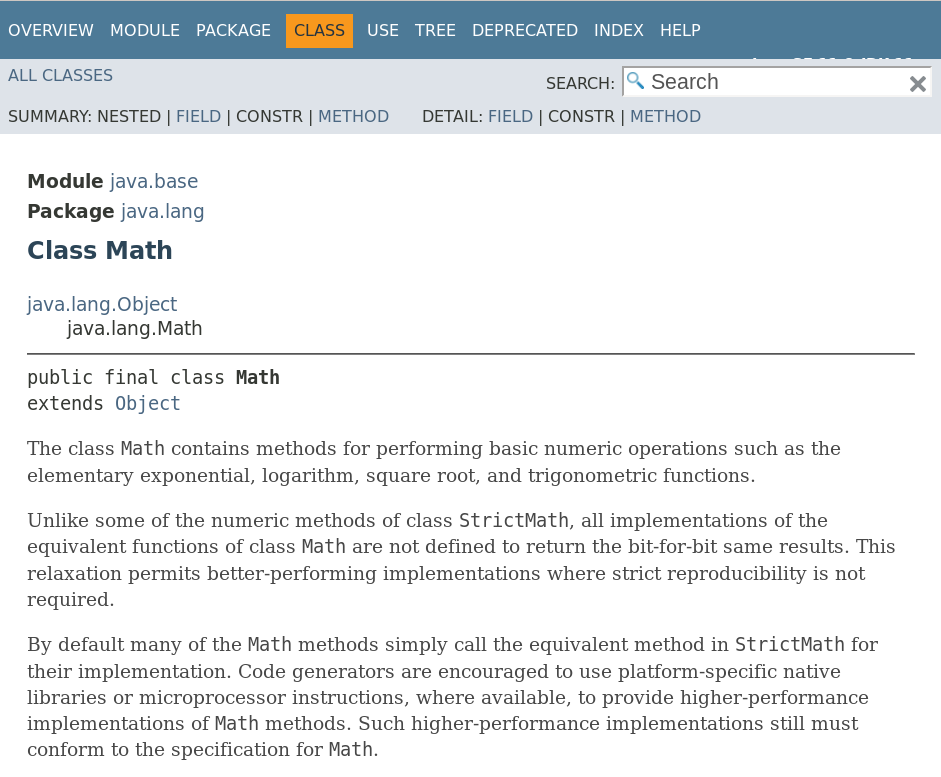
\includegraphics[width=.9\linewidth]{images/javadoc-math.png}
	\caption{Exemple~: le haut de page de la documentation de la classe \pc{Math} pour JDK11}
	\label{fig:javadocmath}
\end{figure}

Cette description de la classe est suivie de la liste des méthodes de la classe
accompagnée de la description courte de chacune d'entre elles. Plus bas se
trouve la description longue de la méthode (voir par exemple la figure
\vref{fig:javadocmathabs}).

\begin{figure}[h]
	\centering
	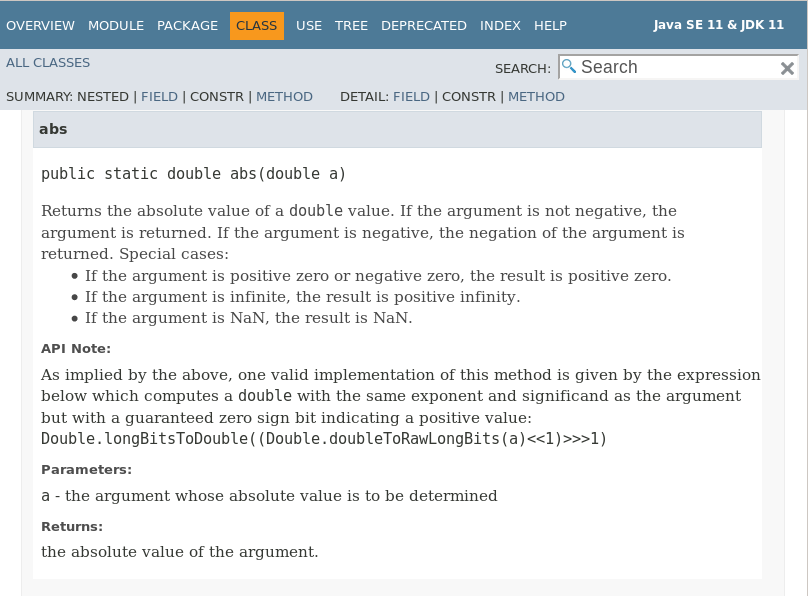
\includegraphics[width=.9\linewidth]{images/javadoc-abs.png}
	\caption{Exemple~: la description longue de la documentation de la méthode \pc{Math.abs} pour JDK11}
	\label{fig:javadocmathabs}
\end{figure}


L'outil \texttt{javadoc} permet l'harmonisation de la documentation Java et la
génération complète de la documentation.  


\section{Le commentaire \texttt{javadoc}}

Comme nous l'avons vu à la section \vref{section:commentaires}, il existe
3 manières d'écrire les commentaires en Java. Seuls les commentaires identifiés
par \pc{/** */} sont destinés à l'outil \pc{javadoc}. 

\index{signature}
\index{declaration}
Le commentaire \textit{javadoc} se place au dessus de la déclaration de la
classe pour la documentation de la classe et au dessus de la déclaration de
chaque méthode pour la documentation des méthodes de la classe. 

Nous reviendrons sur la \textbf{déclaration d'une classe} dans le cours de
Développement~II\footnote{Pour la personne curieuse, la notion de déclaration
d'une classe se trouve dans \cite{jls9} à la section 8.1 }. 

\marginicon{definition}
La \textbf{déclaration de la méthode} se compose~:

\begin{itemize}
	\item des \textit{modifiers} comme \pc{public} et \pc{static}\,;
	\item du type de retour\,;
	\item du nom de la méthode\,
	\item de la liste de ses paramètres\,;
	\item d'une liste éventuelles d'exceptions\,;
	\item du corps de la méthode.
\end{itemize}

Le nom de la méthode et la liste des paramètres forment la \textbf{signature}
de la méthode (cfr. section 8.4.2 de \cite{jls9}). \textit{javadoc} utilise la
signature de la méthode et son type de retour pour générer la documentation.
Sur base des informations contenues dans le commentaire, du type de retour de
la méthode et de sa signature, \textit{javadoc} produit des pages html ayant la
même forme que celles de la documentation officielle de l'API Java.  

\pagebreak
Un commentaire comme~:

\begin{java}
/**
* Description courte de la méthode terminée 
* par un point.
* 
* Un peu plus en détail ce que fait la méthode. La description 
* longue peut contenir des balises html comme <strong>écrire 
* en gras</strong> par exemple. 
* 
* @param par1 rôle du paramètre (son type est déduit)
* @return valeur de retour
*/
public static <Type> <nom>(<params>){
	// Statement
}
\end{java}

produit si l'on choisit \texttt{String} comme type de retour et un paramètre de
type \texttt{int}, une documentation à l'allure de la figure
\vref{fig:javadocdescriptioncourte},

\begin{figure}[h]
	\centering
	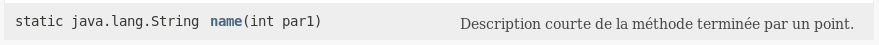
\includegraphics[width=.9\linewidth]{images/javadoc-descriptioncourte.png}
	\caption{Javadoc~: description courte}
	\label{fig:javadocdescriptioncourte}
\end{figure}

à laquelle correspond la description longue de la figure
\vref{fig:javadocdescriptionlongue}.

\begin{figure}[h]
	\centering
	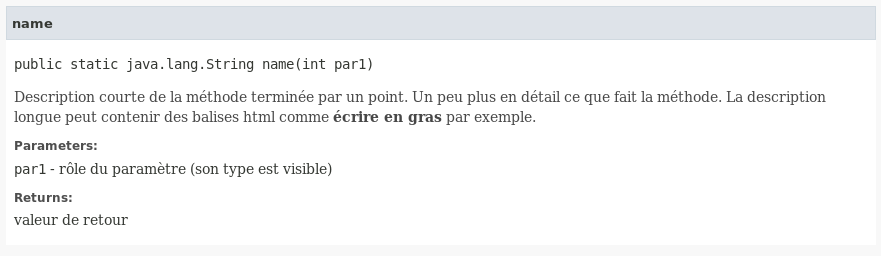
\includegraphics[width=.9\linewidth]{images/javadoc-descriptionlongue.png}
	\caption{Javadoc~: description longue}
	\label{fig:javadocdescriptionlongue}
\end{figure}


\index{tag}
\subsection{Les tags}

Afin de mettre correctement la documentation en forme, \textit{javadoc} utilise
des \textbf{tags}. Ce sont des mots commençant par un \textit{arobase} —~@~—
qui sont reconnus par la commande \texttt{javadoc}. Certains sont requis,
d'autres optionnel.  Certains sont destinés à la documentation de la
classe\footnote{Le terme «~classe~» est ici dans son sens large et comprend~:
les classes, les interfaces et les énumérations comme nous le verrons en
Développement~II} d'autres aux méthodes. 

Nous retiendrons ces \textit{tags} placés idéalement dans cet ordre~:

\begin{description}
	\item[@author] renseignant le ou les auteur·es de la classe. Un \textit{tag} 
		par auteur·e. Dans le cadre d'un développement commun, l'auteur peut 
		être un groupe. Ce tag ne génère pas de \textit{javadoc}, il n'est 
		visible que dans la classe. 
		(\textit{classes}, \textit{requis});
	\item[@version] comprend la date de modification et un numéro de version commençant à 1.1. 
		(\textit{classes}, \textit{requis});

		\par Par exemple \textit{1.39, 1996-01-23}
	\item[@param] décrivant chaque paramètre de la méthode. Il y en a un par paramètre;
		(\textit{méthodes}, \textit{requis});
	\item[@return] décrivant ce que retourne la méthode;
		(\textit{méthodes}, \textit{requis} excepté si la méthode ne retourne rien);
	\item[@throws] listant les exceptions éventuellement lancées par la méthode;
		(\textit{méthodes});
	\item[@see] renseignant une autre classe ou une autre méthode relative à ce qui est documenté. 
\end{description}



\subsection{Le style}

Voici quelques règles de style\footnote{Ces règles sont principalement issues de \url{https://www.oracle.com/technetwork/java/javase/documentation/index-137868.html}.} pour la rédaction de la \textit{javadoc}.

\begin{enumerate}
	
	\item Seules les classes et les méthodes publiques sont commentées. 

	\item Dans la mesure du possible la \textit{javadoc} s'écrit en anglais. 

	\item Les mots clés (\textit{keywords}), les noms de classes, de méthodes
		sont écrit entre les balises \texttt{<code> </code>} 

	\item On préfèrera la $3^e$ personne à la $2^e$ personne. 

	\item La description d'une méthode commence par un verbe parce qu'elle
		implémente habituellement une opération, une action. 
	
		\medskip 
		\textit{Gets the label of this button.} \\
		sera préféré à \\
		\textit{This method gets the label of this button.}

	\item Ajouter le commentaire au nom de la méthode sans répéter le nom de la
		méthode. Normalement le nom de la méthode est choisi pour représenter
		ce qu'elle fait. Il est donc inutile de répéter ces mots dans la
		documentation. La documentation doit idéalement apporter une plus-value
		au nom de la méthode. 

		\medskip
		Éviter cette description qui ne fait que répéter les mots contenus 
		dans le nom de la méthode.
		\marginicon{dont}
		\begin{java}
		/**
		  * Sets the tool tip text.
		  *
		  * @param text the text of the tool tip
		  */
		  public void setToolTipText(String text)
		\end{java}
		
		Préférer cette description qui définit ce qu'est une infobulle 
		(\textit{tool tip}) dans un contexte plus large. 
		\begin{java}
		/**
		  * Registers the text to display in a tool tip. 
		  * 
		  * The text displays when the cursor lingers over 
		  * the component.         
		  *
		  * @param text the string to display. If the text 
		  * is null, the tool tip is turned off for 
		  * this component. 
		  */
		  public void setToolTipText(String text)
		\end{java}

	\item Le tag \texttt{@link} peut être utilisé… avec parcimonie car un lien
		attire l'attention. Il ne faut pas en abuser. Ce tag s'écrit dans le
		texte et fait référence vers l'API.

	\item Lorsqu'une référence à une autre méthode est faite, on omet les
		parenthèses \texttt{add} ou on écrit le type des paramètres
		\texttt{add(int, Object)} sans nom pour les paramètres. 

	\item Lors de la description éventuelle d'une variable, omettre le sujet
		dans un soucis de brièveté. 

		\medskip
		\textit{Counter of vowels}\\
		sera préféré à\\
		\textit{This is a counter of vowels}.

	\item Éviter les abréviations qui pourraient ne pas être comprises par tous
		et toutes. 

\end{enumerate}







\section{L'outil \texttt{javadoc}}

Il est possible de générer la \textit{javadoc} d'un simple clic à partir d'un IDE comme il est possible de le faire à partir d'une console par~:

\begin{term}
	javadoc MyClass.java
\end{term}

Certaines options sont intéressantes~:

\begin{description}

	\item[-d <directory>] demande de générer la documentation dans le
		répertoire \texttt{directory} plutôt que dans le répertoire courant.
		Crée le répertoire au besoin;

	\item[-charset utf-8] ajoute du code html permettant la prise en charge de
		l'utf-8 ce qui aura pour effet que les caractères accentués seront
		correctement affichés dans la documentation. 

	\item[-sourcepath <directory>] précise dans quels répertoires chercher les
		fichiers sources lorsque l'on précise le \textit{package} à documenter.
		Par défaut, cherche dans le répertoire courant. Les nom de répertoires
		sont séparés par deux points ($:$) s'il y en a plusieurs.

\end{description}

\textbf{Exemples:}

Tous mes fichiers sources se trouvent dans le sous répertoire \texttt{src}, je
génère la documentation en une seule fois dans le répertoire \texttt{doc} par~:

\begin{term}
	javadoc src/*.java -d doc -charset utf-8
\end{term}

Mes fichiers sources sont dans un répertoire \texttt{src} et dans des
sous-répertoires, je peux demander à mon shell de les chercher avant d'en
fournir la liste à \texttt{javadoc}. Je génère la documentation dans le répertoire \texttt{doc} par~:

\begin{term}
	javadoc \$(find src -name '*.java') -d doc -charset utf-8 
\end{term}

Mes classes font toutes partie du \textit{package}\footnote{La notion sera vue en Développement II, à ce stade, supposont que les classes ont toutes la même instruction \texttt{package} en début de fichier} \texttt{my.package} et se trouve dans le répertoire \texttt{src/my/package/}. Je génère la documentation dans le répertoire \texttt{doc} par~:

\begin{term}
javadoc my.package -d doc -charset utf-8 -sourcepath src
\end{term}



